% !TeX root = main.tex
% !TeX program = xelatex
% !TeX options = -synctex=1 -interaction=nonstopmode -file-line-error "%DOC%"

\documentclass[aspectratio=169]{beamer}

\usepackage{tikz}
\usetikzlibrary{calc}
\usepackage{kotex}
\usepackage{fmtcount}
\usepackage{fontspec}
    \setmainfont{NotoSans}[
        UprightFont = {*-Regular},
        BoldFont = {*-Bold},
        ItalicFont = {*-Italic},
        BoldItalicFont = {*-BoldItalic},
        Path = {./fonts/},
        Extension = {.ttf}
    ]
    \setsansfont{NotoSans}[
        UprightFont = {*-Regular},
        BoldFont = {*-Bold},
        ItalicFont = {*-Italic},
        BoldItalicFont = {*-BoldItalic},
        Path = {./fonts/},
        Extension = {.ttf}
    ]
    \setmainhangulfont{NotoSansKR}[
        UprightFont = {*-Regular},
        BoldFont = {*-Bold},
        % ItalicFont = {*-Italic},
        Path = {./fonts/},
        Extension = {.otf}
    ]
    \setsanshangulfont{NotoSansKR}[
        UprightFont = {*-Regular},
        BoldFont = {*-Bold},
        % ItalicFont = {*-Italic},
        Path = {./fonts/},
        Extension = {.otf}
    ]

\definecolor{primary-color}{RGB}{232, 100, 62}

\usetheme{Ansi}

\title{신입생\\\textbf{C언어}\\스터디}
\subtitle{Hello, world!}
\author{Jisu Sim}
\institute{소프트웨어학과 소학회 A.N.S.I.}
\chapternumber{1}

\def\nextchapter{변수와 자료형}

\begin{document}

%%%%%%%%%%%%%%%%%%%%%%%%%%%%%%%%%%%%%%%%%%%%%%%%%%%%%%%%%%%%%%%%%%%%%%%%%%%%%%%%
% 표지
%%%%%%%%%%%%%%%%%%%%%%%%%%%%%%%%%%%%%%%%%%%%%%%%%%%%%%%%%%%%%%%%%%%%%%%%%%%%%%%%
\begin{frame}[plain]
    \titlepage
\end{frame}

%%%%%%%%%%%%%%%%%%%%%%%%%%%%%%%%%%%%%%%%%%%%%%%%%%%%%%%%%%%%%%%%%%%%%%%%%%%%%%%%
% 목차
%%%%%%%%%%%%%%%%%%%%%%%%%%%%%%%%%%%%%%%%%%%%%%%%%%%%%%%%%%%%%%%%%%%%%%%%%%%%%%%%
\begin{frame}{목차}
    \tableofcontents
\end{frame}

%%%%%%%%%%%%%%%%%%%%%%%%%%%%%%%%%%%%%%%%%%%%%%%%%%%%%%%%%%%%%%%%%%%%%%%%%%%%%%%%
% 소개
%%%%%%%%%%%%%%%%%%%%%%%%%%%%%%%%%%%%%%%%%%%%%%%%%%%%%%%%%%%%%%%%%%%%%%%%%%%%%%%%
\section{소개}

\begin{frame}[plain]
    \sectionpage
\end{frame}

\begin{frame}{소개}
    여기에 소개에 대한 내용이 들어갑니다
    \begin{enumerate}
        \item 이렇게
        \item 목록을
        \item 적을 수
        \item 있습니다.
    \end{enumerate}
\end{frame}

%%%%%%%%%%%%%%%%%%%%%%%%%%%%%%%%%%%%%%%%%%%%%%%%%%%%%%%%%%%%%%%%%%%%%%%%%%%%%%%%
% 테스트
%%%%%%%%%%%%%%%%%%%%%%%%%%%%%%%%%%%%%%%%%%%%%%%%%%%%%%%%%%%%%%%%%%%%%%%%%%%%%%%%
\section{테스트}

\begin{frame}[plain]
    \sectionpage
\end{frame}

\begin{frame}{테스트}
    테스트 테스트 테스트
    \begin{enumerate}
        \item 이렇게
        \item 목록을
        \item 적을 수
        \item 있습니다.
    \end{enumerate}
\end{frame}

%%%%%%%%%%%%%%%%%%%%%%%%%%%%%%%%%%%%%%%%%%%%%%%%%%%%%%%%%%%%%%%%%%%%%%%%%%%%%%%%
% 마무리
%%%%%%%%%%%%%%%%%%%%%%%%%%%%%%%%%%%%%%%%%%%%%%%%%%%%%%%%%%%%%%%%%%%%%%%%%%%%%%%%
\section{마무리}

\begin{frame}[plain]
    \begin{tikzpicture}[remember picture, overlay]
        \node[above right, inner sep = 0pt] at (current page.south west) {
            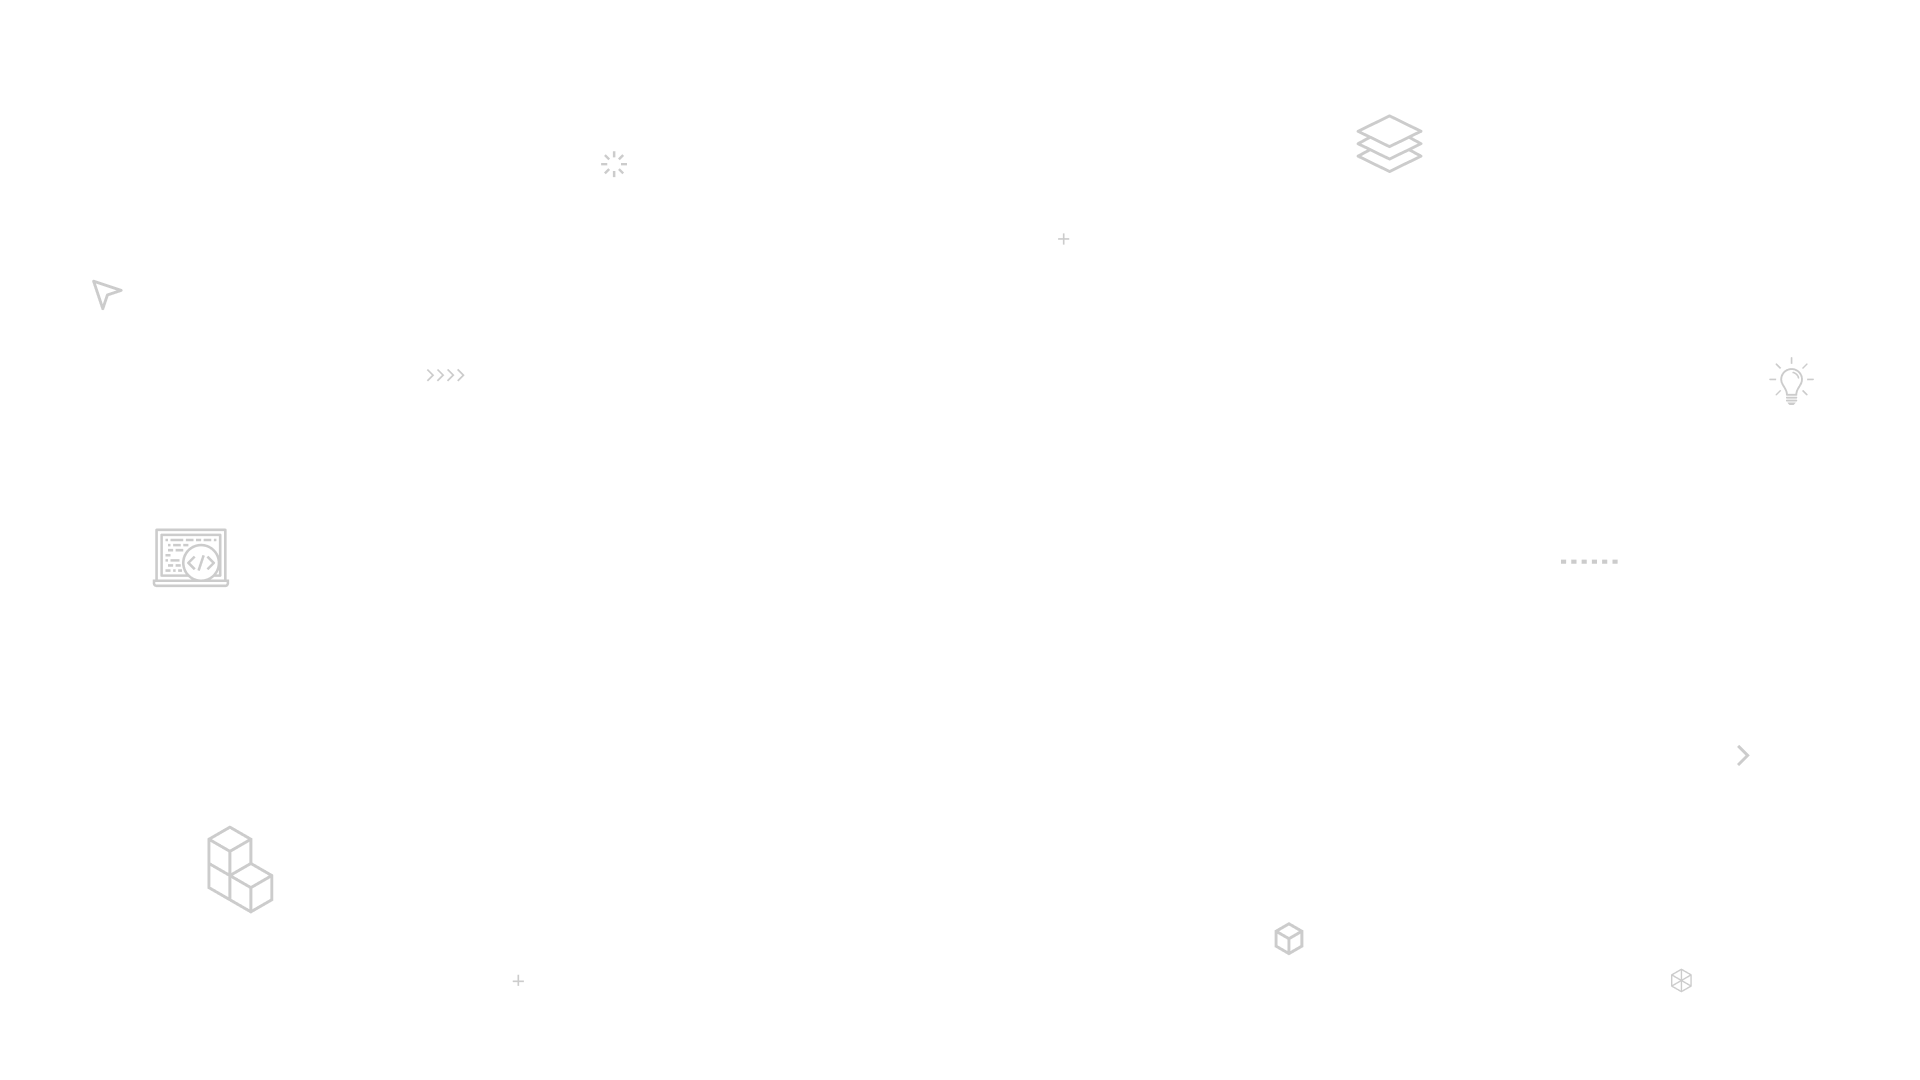
\includegraphics[width=\paperwidth, height=\paperheight]{images/background-white.png}
        };
        \node[anchor=south] at (current page.center) {
            {%
                \fontsize{28}{28}\selectfont%
                \color{primary-color}{%
                    \textbf{수고하셨습니다}%
                }%
            }%
        };
        \node[anchor=north] at (current page.center) {
            다음 강의는 \nextchapter 입니다
        };
    \end{tikzpicture}
\end{frame}

\end{document}